% Project XXXXXXX
%
%%%%%%%%%%%%%%%%%%%%%%%%%%%%%%%%%%%%%%%%%%%%%%%%%%%%%%%%%%%%%%%%%%%%%%%%%%%%%%%
% Set a class and general configuration
\documentclass[11pt,a4paper,oneside]{book}

%%%%%%%%%%%%%%%%%%%%%%%%%%%%%%%%%%%%%%%%%%%%%%%%%%%%%%%%%%%%%%%%%%%%%%%%%%%%%%%
% Set variables with the title, authors, etc.
\newcommand{\Title}{Projeto de estágio docente}
\newcommand{\Year}{2023}
\newcommand{\Date}{Setembro de \Year{}}
\newcommand{\Author}{Leonardo Uieda}

%%%%%%%%%%%%%%%%%%%%%%%%%%%%%%%%%%%%%%%%%%%%%%%%%%%%%%%%%%%%%%%%%%%%%%%%%%%%%%%
% Import the required packages
\usepackage[utf8]{inputenc}
\usepackage[TU]{fontenc}
\usepackage[brazil]{babel}
\usepackage{amsmath}
\usepackage{amssymb}
\usepackage{graphicx}
\usepackage{hyperref}
\usepackage{fancyhdr}
\usepackage{geometry}
\usepackage{booktabs}
\usepackage{microtype}
\usepackage{siunitx}
\usepackage{xcolor}
% Improved urls with proper hyphenation
\usepackage{xurl}
% Tweak the look of captions
\usepackage{caption}
% To control the style of section titles
\usepackage{titlesec}
% Import natbib and doi packages
\usepackage[round,authoryear,sort]{natbib}
% Add the bibliography to the table of contents
\usepackage[nottoc,chapter]{tocbibind}
% Reference sections by name
\usepackage{nameref}
% Better handling of footnotes inside summary boxes
\usepackage{footmisc}
% Show dois as links on references
\usepackage{doi}
% Remove extra space between references
\usepackage{natbibspacing}
% Use a different font
\usepackage[scaled=0.9,sfdefault]{notomath}
% Icons and fonts (requires using xelatex or luatex)
\usepackage{fontawesome5}
\usepackage{academicons}
% Control the font size
\usepackage{anyfontsize}
\usepackage{setspace}
% To get the number of pages in the document
\usepackage{lastpage}
\usepackage{ragged2e}
% Control over enumerate and itemize
\usepackage{enumitem}
% To define custom environments
\usepackage{environ}
\usepackage{mdframed}
% To control hyphenation for individual blocks of text
\usepackage{hyphenat}
\usepackage{lipsum}

%%%%%%%%%%%%%%%%%%%%%%%%%%%%%%%%%%%%%%%%%%%%%%%%%%%%%%%%%%%%%%%%%%%%%%%%%%%%%%%
% Configuration of the document

\geometry{%
  left=25mm,
  right=25mm,
  top=20mm,
  bottom=15mm,
  headsep=0mm,
  headheight=0mm,
  footskip=7mm,
  includehead=true,
  includefoot=true
}

% Control line and table row spacing
\onehalfspacing
\renewcommand{\arraystretch}{1.5}

% Make urls use the same font as every other text
\urlstyle{same}

% Set the spacing between bibliography entries (requires natbib)
\setlength{\bibsep}{0pt}

% Prevent footnotes from being broken into multiple pages
\interfootnotelinepenalty=10000

% Customize how Chapter headings are displayed
\titleformat{\chapter}[display]{\normalfont}{\large Parte \thechapter}{0pt}{\huge\onehalfspacing}[\titlerule]
\titlespacing*{\chapter}{0pt}{-20pt}{20pt}

% Custom colors
\definecolor{darkgray}{gray}{0.4}
\definecolor{mediumgray}{gray}{0.5}
\definecolor{lightgray}{gray}{0.9}
\definecolor{mediumblue}{HTML}{2060c2}
\definecolor{lightblue}{HTML}{f7faff}

% Configure captions
\captionsetup[table]{position=below,skip=0pt}
\captionsetup{labelfont=bf,font={small,color=darkgray},skip=10pt}

% Configure hyperref and add PDF metadata
\hypersetup{
    colorlinks,
    allcolors=mediumblue,
    pdftitle={\Title},
    pdfauthor={\Author},
    breaklinks=true,
}

% Configure header and footer
% Inspired by LaPreprint: https://github.com/roaldarbol/LaPreprint
\renewcommand{\chaptermark}[1]{\markboth{#1}{}}
\newcommand{\Separator}{\hspace{3pt}|\hspace{3pt}}
\newcommand{\FooterFont}{\footnotesize\color{mediumgray}}
\pagestyle{fancy}
\fancyhf{}
\lfoot{%
  \FooterFont{}
  \leftmark{}
}
\rfoot{%
  \FooterFont{}
  \thepage\space de\space \pageref*{LastPage}
}
\renewcommand{\headrulewidth}{0pt}
\renewcommand{\footrulewidth}{1pt}
\preto{\footrule}{\color{lightgray}}
\fancypagestyle{plain}{%
  \fancyhf{}
  \cfoot{%
    \FooterFont{}
    \Title{}
    \Separator{}
    \Author{}
  }
}

% Define fancy text boxes
\NewEnviron{summarybox}[1]{%
  \mdfdefinestyle{summarybox_}{%
    leftline=true,
    rightline=false,
    topline=false,
    bottomline=false,
    linewidth=3pt,
    linecolor=mediumblue,
    backgroundcolor=lightblue,
    innertopmargin=12pt,
    innerbottommargin=12pt,
    innerleftmargin=12pt,
    innerrightmargin=12pt,
    skipbelow=15pt,
    skipabove=15pt,
    frametitleaboveskip=12pt,
    frametitlebelowskip=5pt,
  }
  \newmdenv[style=summarybox_]{summarybox_}
  \begin{summarybox_}[frametitle=#1]
    \BODY
  \end{summarybox_}
}

% Make a list with no margin and smaller spacing for use with the summaryboxes
\NewEnviron{listnomargin}[1]{%
  % Remove spacing between enumerate/itemize items
  \setlist{nosep}
  \begin{#1}[leftmargin=*]
    \BODY
  \end{#1}
}

%%%%%%%%%%%%%%%%%%%%%%%%%%%%%%%%%%%%%%%%%%%%%%%%%%%%%%%%%%%%%%%%%%%%%%%%%%%%%%%
\begin{document}

\pagestyle{empty}
\frontmatter

\begin{titlepage}
  \begin{center}
    
\includegraphics[height=1cm]{figures/usp.png}
    \hfill
    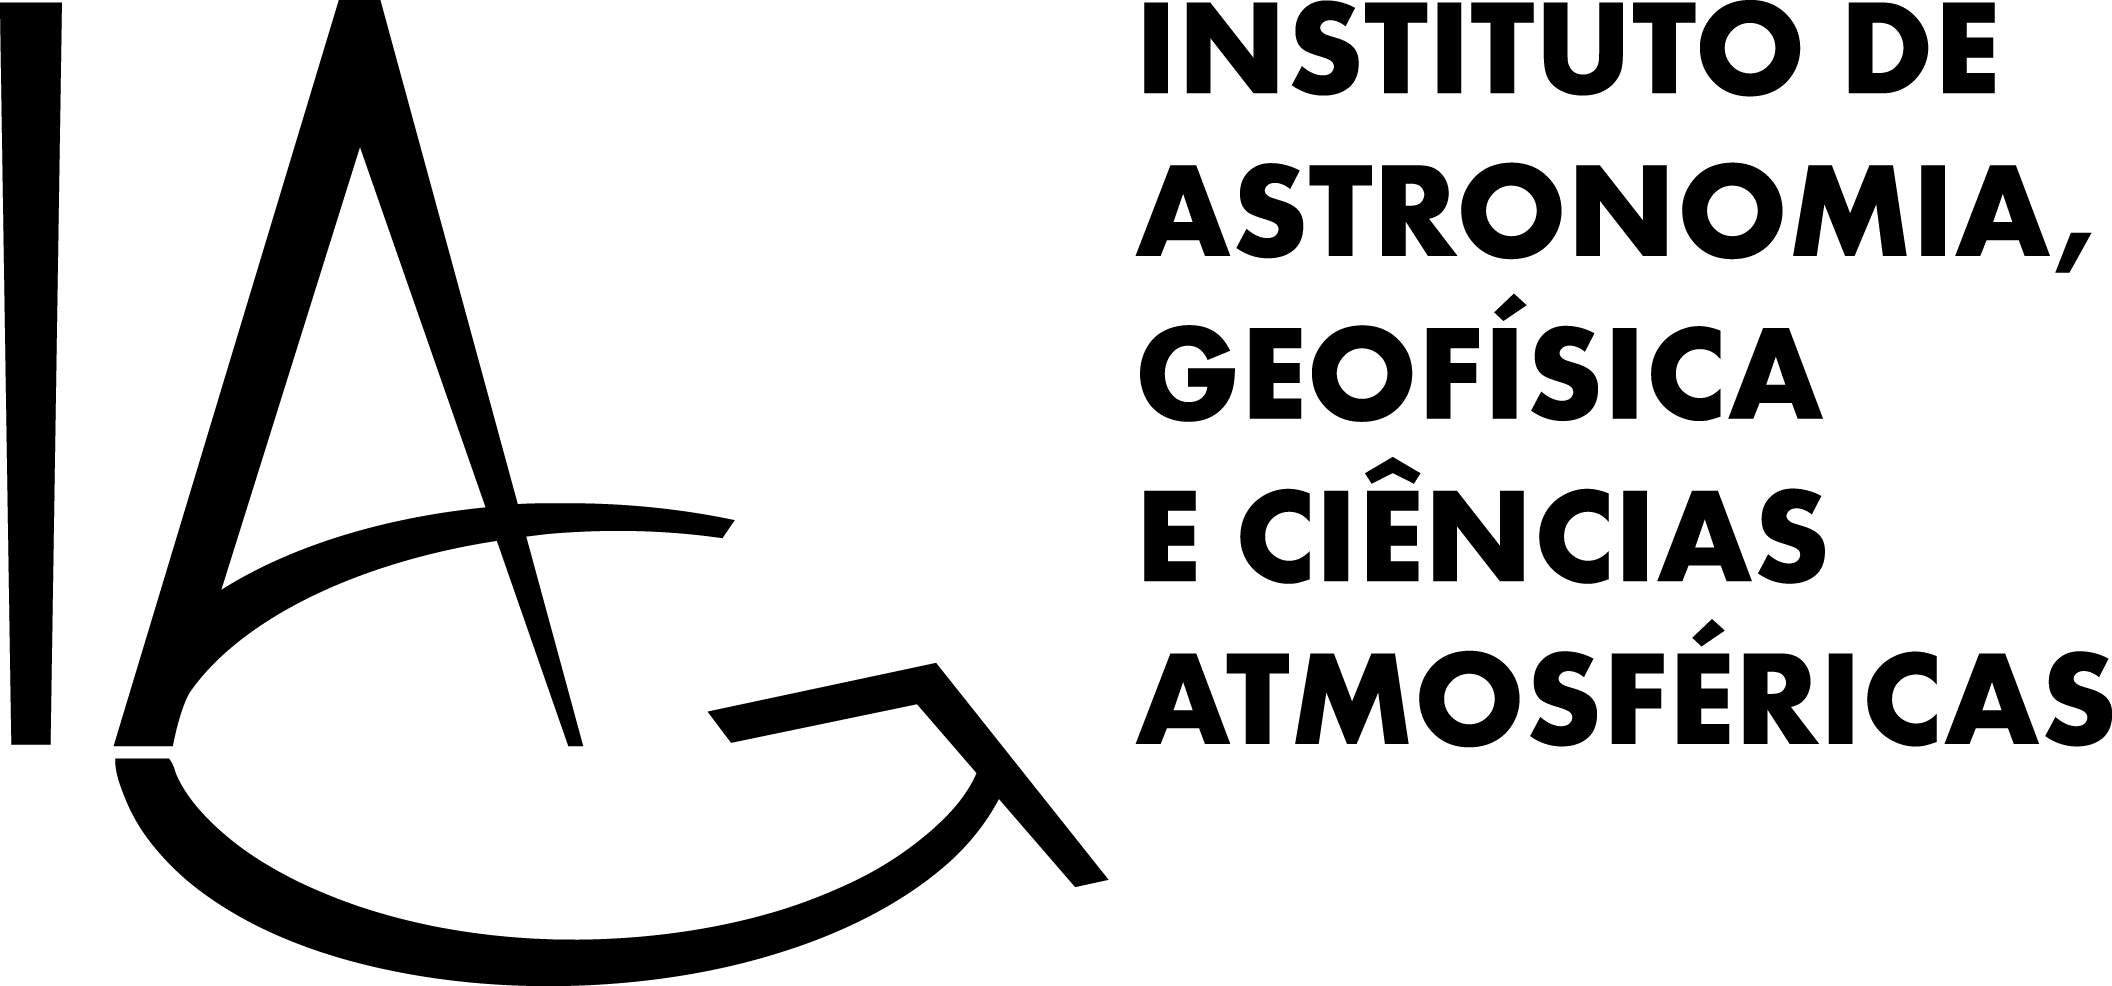
\includegraphics[height=1cm]{figures/iag.png}
    \vspace{9cm}

    \textbf{\Huge \MakeUppercase{\Title{}}}
    \vspace{2cm}

    \textbf{\LARGE \Author{}}
    \vfill

    Departamento de Geofísica
    \\
    Instituto de Astronomia, Geofísica e Ciências Atmosféricas
    \\
    Universidade de São Paulo
    \vspace{2cm}

    \Date{}
  \end{center}
\end{titlepage}

\tableofcontents

\mainmatter
\pagestyle{fancy}

%==============================================================================
\chapter{Introdução}

Durante a minha carreira, atuei em diversas linhas de pesquisa relacionadas a
problemas inversos em métodos potenciais.

%==============================================================================
\chapter{Extensão e cultura}

Feira de profissões.

Curso de verão.

Workshop simpeg/fatiando juntando academia e indústria.

%==============================================================================
\chapter{Funções de gestão universitária}

Comissão de Cooperação Nacional e Internacional

%==============================================================================
\chapter{Pesquisa}

Resumo


\section{%
  Projeto: Integração de dados magnéticos aéreos e de satélite para a
  determinação do fluxo geotermal Antártico
}

\subsection{Enunciado do problema}
% Qual será o problema tratado pelo projeto e qual sua importância? Qual será a
% contribuição para a área se bem-sucedido? Cite trabalhos relevantes na área,
% conforme necessário.

O fluxo geotermal, que é a taxa de variação vertical de calor vindo da
crosta terrestre, é considerado um importante fator que influencia a evolução
das geleiras na Antártica \citep{Seroussi2017}.
Um grande esforço tem sido feito recentemente pela comunidade científica para
melhor entender a variação espacial do fluxo geotermal antártico e seu papel
durante esse período de mudanças climáticas \citep{BurtonJohnson2020}.
Porém, o fluxo geotermal nas regiões polares ainda é pouco conhecido devido à
dificuldade de se obter medições diretas desse parâmetro no ambiente hostil no
interior do continente antártico \citep{BurtonJohnson2020}.
Com a escassez de medições diretas, se torna necessário estimar o fluxo
geotermal na base das geleiras utilizando a geofísica, como a tomografia
sísmica, a magnetometria e a gravimetria.
Dados magnéticos são frequentemente usados, tanto provenientes de aquisições
aéreas \citep[e.g.,][]{Lowe2023} quanto de satélites
\citep[e.g.,][]{FoxMaule2005}.

A relação entre as anomalias magnéticas provindas da litosfera terrestre e o
fluxo geotermal na superfície é indireta e depende de diversas premissas.
Assumindo que a magnetização da crosta se dá numa direção próxima à do campo
geomagnético (i.e., a magnetização é predominantemente induzida), é possível
estimar a profundidade máxima das fontes magnéticas \citep{Spector1970}.
Essa profundidade nos informa onde as rochas atingem a temperatura de Curie,
na qual os minerais ferromagnéticos perdem sua capacidade de armazenar
magnetização e se tornam paramagnéticos com uma baixa susceptibilidade
magnética \citep{Blakely1988}.
Se as fontes magnéticas forem compostas do mineral magnetita, podemos então
deduzir que uma isoterma de aproximadamente \qty{580}{\degreeCelsius} (a
temperatura de Curie da magnetita) se encontra na profundidade estimada.
Sabendo a temperatura em profundidade e na superfície, podemos finalmente
estimar o fluxo geotermal na superfície $q_z$ utilizando uma aproximação para a
Lei de Fourier

\begin{equation}
  q_z = c_t \dfrac{\partial T}{\partial z} \approx c_t \dfrac{T_s - T_c}{\Delta z_c},
\end{equation}

\noindent
onde $c_t$ é a condutividade térmica das rochas, $T$ é a temperatura, $z$ é a
coordenada vertical, $\Delta z_c$ é a profundidade da isoterma de Curie (obtida
através dos dados magnéticos) e $T_s$ e $T_c$ são a temperatura na superfície e
a temperatura de Curie, respectivamente.
Nesta equação se encontra a última premissa deste processo: assume-se que a
condutividade térmica das rochas é uniforme e que seu valor é conhecido.

A classe de métodos mais popular para se obter a profundidade da isoterma de
Curie a partir de dados magnéticos utiliza uma relação estatística entre o
espectro de amplitudes dos dados e a profundidade das fontes magnéticas
\citep{BurtonJohnson2020}.
Essa relação foi estabelecida por \citet{Spector1970} para obter uma
profundidade média do topo e da base do conjunto de fontes magnéticas em uma
área.
Desde então, o método foi aprimorado por diversos autores \citep[uma revisão
dos métodos e suas limitações pode ser encontrada em ][]{NunezDemarco2020}.
Para obter uma distribuição espacial das profundidades, alguns trabalhos
dividem a área de investigação em janelas com uma certa sobreposição e estimam
a profundidade das fontes dentro de cada janela.
Os métodos derivados de \citet{Spector1970} se tornaram ubíquos devido a sua
simplicidade e eficiência computacional.
Porém, existem críticas do uso indiscriminado do método
\citep{Johnson2016,NunezDemarco2020}.
Por exemplo, \citet{Johnson2016} recomendam seu uso somente como uma estimativa
inicial das características gerais da área de investigação antes de se utilizar
métodos mais sofisticados de modelagem direta e inversa.

Não é difícil prever que a incerteza das estimativas de fluxo geotermal a
partir de dados magnéticos será grande, envolvendo erros na compilação dos
dados aeromagnéticos e também as limitações do método em si
\citep{BurtonJohnson2020}.
Estudos recentes utilizando dados magnéticos para aprendizagem de máquinas
\citep{Losing2021} e para reconstruções paleogeográficas \citep{Ebbing2021} tem
apresentado resultados promissores.
\citet{Ebbing2021} sugerem que a integração de dados de satélite e
aeromagnéticos é necessária, enquanto \citet{Lowe2023} argumentam que a alta
resolução dos dados de aerolevantamentos devem ser preservadas.
Os dados magnéticos também são utilizados para treinar os algoritmos de
aprendizagem de máquinas.
Logo, esses dados necessitam ser de alta qualidade para obter previsões
confiáveis.

Considerando os pontos descritas acima, fica claro que é essencial obter novas
formas de:

\begin{enumerate}
  \item Integrar dados de satélite e aerolevantamentos para providenciar uma
    cobertura total do continente e, ao mesmo tempo, preservar a alta resolução
    dos dados aeromagnéticos.
  \item Transformar dados da anomalia magnética do campo total em quantidades
    que sejam menos sensíveis à direção de magnetização das fontes, como a
    amplitude do campo magnético anômalo \citep{Melo2021}. Lembrando que os
    métodos para obter a profundidade da isoterma de Curie assumem conhecimento
    sobre a direção de magnetização das fontes.
  \item Estimar a profundidade da isoterma de Curie a partir de dados
    magnéticos utilizando métodos mais sofisticados de inversão,
    preferencialmente em uma aproximação esférica da Terra devido ao tamanho da
    Antártica.
\end{enumerate}

% Qual será o problema tratado pelo projeto e qual sua importância? Qual será a
% contribuição para a área se bem-sucedido? Cite trabalhos relevantes na área,
% conforme necessário.
\noindent
Neste projeto, iremos desenvolver métodos numéricos e ferramentas
computacionais abertas para resolver essas questões.
As soluções encontradas poderão levar a novos entendimentos sobre a estrutura
crustal e evolução tectônica da Antártica, sobre as limitações do uso de dados
magnéticos mesmo com métodos novos de processamento e também sobre os fatores
que controlam o fluxo geotermal embaixo das geleiras.

\begin{summarybox}{\faBullseye{} Objetivos principais}
  \begin{listnomargin}{enumerate}
    \item Combinar todos os dados magnéticos de satélite e aéreos disponíveis
      para a Antártica em um novo conjunto de dados com espaçamento e altitude
      uniformes.
    \item Transformar os dados de anomalia magnética de campo total ($\Delta
      T$) em dados de amplitude total do campo magnético anômalo
      ($\|\mathbf{B}\|$), que são menos sensíveis à variações na direção de
      magnetização das fontes.
    \item Utilizar os novos dados de amplitude total do campo para estimar a
      profundidade da isoterma de Curie e o fluxo geotermal na base das
      geleiras antárticas.
  \end{listnomargin}
\end{summarybox}

\subsection{Resultados esperados}
% O que será criado ou produzido como resultado o projeto proposto?

Este projeto está divido em três epatas:

\begin{itemize}
  \item \textbf{Etapa 1:} Integração de dados magnéticos utilizando fontes
    equivalentes.
  \item \textbf{Etapa 2:} Transformação de dados de anomalia magnética de campo
    total em dados de amplitude do campo magnético anômalo utilizando fontes
    equivalentes.
  \item \textbf{Etapa 3:} Estimativa da profundidade da isoterma de Curie
    utilizando um método de inversão não-linear em uma aproximação esférica.
\end{itemize}

\noindent
Esperamos que este projeto produza os seguintes resultados:

\begin{enumerate}
  \item Uma nova maneira de integrar dados magnéticos de satélite e de
    levantamentos aerogeofísicos utilizando o método de
    \textit{gradient-boosted equivalent sources} \citep{Soler2021} com uma
    resolução nunca antes alcançada [etapa 1].
  \item Conhecimento proveniente de resultados experimentais sobre as vantagens
    e limitações do uso da \textit{amplitude do campo magnético anômalo} no
    contexto antártico para a interpretação geológica \citep{Melo2021} e a
    recuperação da profundidade da isoterma de Curie \citep{HidalgoGato2021}
    [etapas 2 e 3].
  \item Um novo método de inversão, baseado em \citet{Uieda2017} e
    \citet{HidalgoGato2021}, para estimar a profundidade da isoterma de Curie
    em uma aproximação esférica da Terra a partir de dados da amplitude do
    campo magnético anômalo e com vínculos provenientes de outros dados
    geofísicos [etapa 3].
  \item Uma nova estimativa da isoterma de Curie e do fluxo geotermal com maior
    resolução espacial e consistência com outras estimativas [etapa 3].
\end{enumerate}

\noindent
Além disso, o projeto também poderá gerar os seguintes recursos para a
comunidade científica, todos disponibilizados gratuitamente sob licenças
abertas:

\begin{enumerate}
  \item Componentes adicionadas ao software livre Harmonica para:
    1) a combinação de dados magnéticos e a sua transformação em dados de
       amplitude do campo anômalo utilizando fontes equivalentes [etapas 1 e
       2];
    2) a inversão dos dados magnéticos em coordenadas esféricas para estimar a
       profundidade da isoterma de Curie [etapa 3].
  \item Uma nova compilação de dados magnéticos para a Antártica na forma de
    uma malha regular com altitude controlada cobrindo todo o continente e os
    oceanos adjacentes [etapas 1 e 2].
\end{enumerate}

\subsection{Desafios científicos e tecnológicos}
% Explicite os desafios científicos e tecnológicos que o projeto se propõe a
% superar para atingir os objetivos. Descreva com que meios e métodos estes
% desafios poderão ser vencidos. Cite referências que ajudem os assessores que
% analisarão a proposta a entenderem que os desafios mencionados não foram
% ainda vencidos (ou ainda não foram vencidos de forma adequada) e que poderão
% ser vencidos com os métodos e meios da proposta em análise.

\subsection{Disseminação e avaliação}
% Como os resultados do projeto deverão ser avaliados e como serão
% disseminados?

Os resultados provenientes deste projeto serão avaliados utilizando:

\begin{itemize}
  \item Testes com dados sintéticos utilizando modelos geologicamente
    plausíveis. Nestes testes, sabemos qual é o resultado esperado e então
    podemos calcular o erro cometido pelos métodos desenvolvidos. Através de
    dados sintéticos, podemos também avaliar as limitações dos métodos e ganhar
    experiência para diagnosticar problemas que podem ocorrer na aplicação a
    dados reais.
  \item Comparação com resultados anteriores. Por exemplo, as compilações de
    dados magnéticos ADMAP-2 e ADMAP-2s \citep{Golynsky2018, Kim2022} e outros
    modelos de fluxo geotermal \citep{FoxMaule2005, Losing2021, Losing2020,
    Stal2021}.
\end{itemize}

\noindent
A disseminação dos resultados será feita através de:

\begin{itemize}
  \item Artigos em periódicos internacionais.
  \item Campanhas em mídias sociais no formato de e-pôsteres.
  \item Apresentação dos resultados em congressos internacionais da EGU, AGU e
    SCAR.
  \item Tutoriais em formato de páginas na internet e vídeos que explicam como
    utilizar os métodos desenvolvidos para outras aplicações.
  \item Vídeos de divulgação científica para o público geral. Criadores com
    audiência estabelecida na plataforma YouTube (por exemplo,
    \href{https://www.youtube.com/@MinuteEarth}{MinuteEarth} ou
    \href{https://www.youtube.com/@manualdomundo}{Manual do Mundo})
    serão contratados para produzir os vídeos\footnote{Um exemplo disso é este
    vídeo, que tem mais de meio de milhão de visualizações, feito pelo canal
    MinuteEarth para divulgar os resultados de um projeto da NSF:
    \url{https://youtu.be/J6d0UqY6IsA}}.
\end{itemize}

\subsection{Outros apoios}
% Demonstre outros apoios ao projeto, se houver, em forma de fundos, bens ou
% serviços, mas sem incluir itens como uso de instalações da instituição que já
% estão disponíveis. Note que os autores das propostas selecionadas deverão
% apresentar carta oficial assinada pelo dirigente da instituição,
% comprometendo os recursos e bens adicionais descritos na proposta.


%==============================================================================
\chapter{Atividade didática}

\section{Disciplinas}


\section{Produção de recursos educacionais abertos}


\section{Orientação de estudantes}

Incluir algo sobre isso ser mais que só pesquisa.

Colocar parte de formação extra-curricular e preparo para o mercado de trabalho
fora do setor acadêmico.

%==============================================================================
\backmatter
\bibliographystyle{apalike-doi}
\bibliography{references}
\chaptermark{Referências Bibliográficas}

\end{document}
